\documentclass[sigplan,screen]{acmart}

\setcopyright{none}

\settopmatter{printacmref=false} % Removes citation information below abstract
\renewcommand\footnotetextcopyrightpermission[1]{} % removes footnote with conference information in first column
\pagestyle{plain} % removes running headers

\AtBeginDocument{%
	\providecommand\BibTeX{{%
		\normalfont B\kern-0.5em{\scshape i\kern-0.25em b}\kern-0.8em\TeX}}}

\hyphenation{src-ML}

% Enumerations
\usepackage[inline]{enumitem}

% Better typesetting of consecutive footnotes
\usepackage{fnpct}
% don't switch kerning and punctuation
\setfnpct{dont-mess-around}

% Draw figures
\usepackage{tikz}
% \includegraphs for .tikz files
\usepackage{tikzscale}

% Lay out multiple figures
\usepackage{subcaption}

% Extended control of figure positioning
\usepackage{dblfloatfix}

% Algorithms
\usepackage[noend,noline,boxed]{algorithm2e}
\SetAlCapSkip{1em}
% Python style
\DontPrintSemicolon
\SetStartEndCondition{ }{}{}%
\SetKwIF{If}{ElseIf}{Else}{if}{:}{else if}{else}{end if}%
\SetKwFor{For}{for}{:}{next}%
\SetKw{kwYield}{yield}

% Source code listings
\usepackage{listings}

% Underlined text with linebreaks
\usepackage[normalem]{ulem}

\usepackage{xcolor}

% Convenient references (needs to be loaded after algorithms)
\usepackage[nameinlink]{cleveref}

% ISSUES:
%  - links are red instead of blue (only local)
%  - footnote separation with the above does not work (already longer)
%  - conference is displayed in header (only remote)

% Semantic markup
\newcommand\caps[1]{
	\textsc{#1}%
}
\newcommand\code[1]{
	\texttt{#1}%
}

\newcommand\TODO[1]{
	\textcolor{red}{\textbf{#1}}%
}



\begin{document}

	\title[Downstream Dependency Mining]{Is This Ever Called? Equipping Package Developers with Usage Information Mined from Downstream Dependency Repositories}

\author{Christoph Thiede}
\email{christoph.thiede@student.hpi.de}
\affiliation{%
	\institution{Hasso Plattner Institute}
	\streetaddress{Prof.-Dr.-Helmert-Str. 2 -- 3}
	\city{Potsdam}
	\country{Germany}
	\postcode{14482}
}
\author{Daniel Limberger}
\email{daniel.limberger@hpi.de}
\affiliation{%
	\institution{Hasso Plattner Institute}
	\streetaddress{Prof.-Dr.-Helmert-Str. 2 -- 3}
	\city{Potsdam}
	\country{Germany}
	\postcode{14482}
}
\author{Willy Scheibel}
\email{willy.scheibel@hpi.de}
\affiliation{%
	\institution{Hasso Plattner Institute}
	\streetaddress{Prof.-Dr.-Helmert-Str. 2 -- 3}
	\city{Potsdam}
	\country{Germany}
	\postcode{14482}
}

\renewcommand{\shortauthors}{Christoph Thiede}


	\begin{abstract}

	In the dependency graph of a software ecosystem, \emph{downstream dependencies} are the nodes that depend on a package.
	Other than for upstream dependencies, solutions that provide individual package developers with this kind of information do not yet exist.
	This paper makes two major contributions:
	\begin{enumerate*}[label=(\roman*)]
		\item We propose an approach for mining usage data about npm packages from their downstream dependencies by utilizing a static type analyzer.
		\item We introduce a tool that allows package developers to survey usage samples of their APIs by incorporating the aggregated usage data into an integrated development environment.%
			\footnote{
				All artifacts are available on GitHub under the following URL: \url{https://github.com/LinqLover/downstream-repository-mining}
				\TODO{Insert name and use link to VSCE}
			}
	\end{enumerate*}
	We find that usage data from downstream dependency repositories are a promising source of information for mining software repositories and that they can be useful to support package developers in improving or extending their APIs.

\end{abstract}

	\keywords{mining software repositories, ecosystem call graphs, API usage, type analyzer, npm}

	\maketitle

	\section{Introduction}
\label{sec:introduction}

Open Source software (OSS) solutions have become more and more and important during the last decades.
Especially, this trend has been experiencing an additional updraft due to the ongoing spreading of OSS platforms such as GitHub or GitLab.
Open-source development offers many advantages as opposed to traditional closed-source development, including large numbers of volunteer contributions from the open-source community, increased transparency effects in security-related domains, and a high potential for reusing solutions.
These solutions are usually organized as \emph{packages} each of which attempts to solve an isolated problem and provide a generic interface.
Most commonly, packages are developed in a \emph{code repository} that is managed using a \emph{development platform} (such a \emph{GitHub}\footnote{\url{https://github.com/}}, \emph{GitLab}\footnote{\url{https://gitlab.com/}}, or \emph{Bitbucket}\footnote{\url{https://bitbucket.com/}}) and deployed to a \emph{package repository} using a \emph{package manager} (such as \emph{PyPI}\footnote{\url{https://pypi.org/}} using \emph{pip}\footnote{\url{https://pip.pypa.io/}} for the Python programming language, the \emph{npm registry}\footnote{\url{https://www.npmjs.com/}} for JavaScript/TypeScript, or the \emph{NuGet Gallery}\footnote{\url{https://www.nuget.org/}} for languages from the .NET ecosystem).
Other solutions or packages can then \emph{depend} on existing packages by declaring them in their manifest, i.e., the \code{package.json} file of an npm package, or the \code{requirements.txt} file of a Python project.
These dependency relations form a large directed graph that connects major parts of the software world for each popular programming language ecosystem.

Despite this connectedness by design, however, the development process of many packages is still characterized by an isolated approach:
While OSS developers commonly submit tickets to or contribute patches against \emph{upstream repositories} that they depend on to solve subproblems, the reverse direction of these edges -- called \emph{downstream dependencies} -- is often neglected by package developers when they extend, restructure, or refactor their solutions.
This knowledge deficit can cause a wide range of alignment issues, including poorly suited interfaces \citep{piccioni2013empirical}, unidentified defects \citep{wong2017more}, and compatibility problems \citep{bogart2015breaks}.
Eventually, all these issues impair the capabilities of the global OSS community to build and support high-quality products.
In the following, we also refer to downstream dependencies will shortly as \emph{dependencies}.

To tackle these concerns, in this paper, we propose an approach to extract API usage samples from downstream dependency repositories of individual packages in order to support package developers in surveying usages of their solutions.
We further make these data directly available to package developers by integrating them into an integrated development environment (IDE).

The rest of this paper is organized as follows:
In \cref{sec:related_work}, we give a summary of existing approaches in this field.
In \cref{sec:framework}, we outline the overall conditions and the general approach for our solution to mining downstream dependencies.
In \cref{sec:dependency_collection} and \cref{sec:usage_mining}, we explain our approach for collecting downstream dependency repositories and mining usage data from these repositories in detail, resp.
In \cref{sec:implementation}, we describe an implementation of the proposed approach and our design decisions for displaying usage samples to the user.
In \cref{sec:evaluation}, we examine the fitness of our data mining approach and the usability of the display solution.

	\section{Related work}
\label{sec:related_work}

To our knowledge, the design of proper tooling for improving package developers' knowledge about interface usages in dependencies has not yet attracted significant attention in the scientific community.
Nevertheless, programmatic analysis of dependency graphs and API usage mining are already common techniques in the field of \emph{mining software repositories} (MSR).
\citet{chaturvedi2013tools} provide a broad overview of existing achievements and ongoing research topics in this field.
Besides source code repositories, they also describe various other data sources worthwhile to examine -- including version control systems, telemetry data from IDEs, issue trackers, and discussion platforms -- as well as different directions for evaluating the retrieved data -- such as classifying or ranking repositories, analyzing the evolution of projects, studying development communities, but also inspecting the relationships and dependencies between projects.
In the following, we will consider the different problems that our research issue can be decomposed into.

\subsection{Mining dependencies}
\label{sec:related_work/dependencies}

A common purpose for \emph{analyzing dependency graphs} is to discover transitive (indirect) upstream dependencies of a project and assess their impact on the stability and vulnerability of the project.
This is done by \citet{kikas2017structure} which apply their methodology to the JavaScript, Ruby, and Rust ecosystems and gain statistical insights into the centrality and evolution of these ecosystems.
\citet{decan2018impact} pursue a similar approach in order to measure the spreading of security vulnerabilities along the chain of downstream dependencies.

However, existing research about dependency graphs primarily takes a broad statistical perspective, and researchers often rely on a large corpus of downloaded software repositories \citep{abdalkareem2017developers,katz2020libraries,kikas2017structure}.
% and researchers usually either access certain package registries such as the npm registry that already contain bidirectional dependency data, or they collect large amounts of software repositories from development platforms such as GitHub, extract dependency lists from each repository's metadata, and finally invert all adjacency lists to get the downstream dependencies.
As opposed to this approach, these capacities will not be appropriate for scenarios that are occasionally performed by developers of a single package only.
In this case, developers will often use a public \emph{code search} service such as GitHub code search\footnote{\url{https://docs.github.com/en/github/searching-for-information-on-github}} or Sourcegraph\footnote{\url{https://sourcegraph.com/}} instead.
\citet{liu2020opportunities} survey current methods and trends in code search tools that include, besides simple full-text search, newer approaches such as structural or semantic search queries, code similarity metrics, or Machine Learning methods.

\subsection{Mining usage information}
\label{sec:related_work/usage_information}

Dependency graphs do not provide information about package usage on a finer granularity, so reference insights about single package members such as classes or methods remain unknown.
The process of extracting fine-granular information about all references to individual elements of an interface is often referred to as \emph{API usage analysis}.
A simple approach to this problem is to perform a string search for package names or members in the dependencies \citep{mileva2010mining}.
\citet{qiu2016understanding} propose a more elaborated approach that operates on the AST of each parsed dependency to avoid false positive matches that can be caused by ambivalent identifier names.
A very similar approach is also chosen by \citet{sawant2017fine} who evaluate the collected usage data in order to analyze the historical importance of certain features supported by an API.

However, the precision of ASTs is limited for dynamically typed languages such as JavaScript.
For this reason, a common data structure that can be used to improve type information are \emph{call graphs} that are either \emph{static} (i.e., the result of a theoretical analysis of the source code) or \emph{dynamic} (i.e., empirically recorded during program execution).
While the latter type has a higher potential for including a maximum of contextual information, the former has the advantage of being applicable to a larger probe of source code for that no concrete entry points are available.
There are many solutions that analyze the structure of programs and extract the relevant information to build call graphs:

\citet{collard2013srcml} propose an infrastructure called \caps{srcML} that is aimed to create a unified representation of multilingual source code snippets for arbitrary analysis purposes, including the construction of call graphs.
Another solution is proposed by \citet{bogar2018lightweight} who focus on analyzing multilingual codebases and who utilize an island parser to build call graphs.
Furthermore, \citet{antal2018static} compare several call graph generators for JavaScript.
They also emphasize that for languages supporting dynamic typing or meta-programming mechanisms, static call graph generators have a limited precision by design.

To bring together dependency graphs and call graphs, \emph{ecosystem call graphs} can be constructed by applying call graphs to entire ecosystems, crossing repository boundaries.
\citet{hejderup2018software} propose an approach to do so for the JavaScript/npm ecosystem in which they also model the semantic version numbers of packages and perform an impact analysis for vulnerabilities based on their graph.
\citet{nielsen2021modular} elaborate on this work by developing a call graph generator tailored to this problem that comes with significant improvements in terms of recall and performance; a very similar method is also sketched by \citet{boldi2020fine}.
\citet{wang2020empirical} describe a similar approach for the same ecosystem and apply it to the domain of locating security issues in a project's upstream dependencies.
With \caps{Pr\"azi}, \citet{hejderup2021praezi} also describe their implementation of a dependency-scale call graph for the Rust/Cratesio ecosystem in-depth.
For Java/Maven, \citet{keshani2021scalable} proposes another solution.

After collecting these usage data, additional processing is possible to extract general usage information from the extensive raw data.
Next to straightforward grouping and counting operations, such aggregations can be built by detecting popular \emph{usage patterns} of API features in the downstream dependencies.
\citet{zhong2009mapo} propose a framework to do so that, for instance, finds sequences of API members that are invoked frequently and even uses these patterns for guiding API users by giving them recommendations.
\citet{hanam2019aiding} pursue a different goal in their tool that helps package developers assess the impact of breaking API changes on the functionality of downstream dependencies.

\subsection{Presentation of results}
\label{sec:related_work/presentation}

To establish an adequate developer experience, any collected usage data still need to be presented in a suitable manner.
A common approach for this is a hierarchical and navigatable representation of the collected call tree.
The first form of this representation has been invented as the ``message set'' tool for browsing senders and implementors in an object-oriented system for the Smalltalk programming environment \citep[section~10.1f.]{goldberg1984smalltalk}.
Modern alternatives include the \caps{Stacksplorer} \citep{karrer2011stacksplorer} or \caps{Blaze} \citep{kramer2012blaze} that list next to the currently focused method other methods which are adjacent to this method in the call graph.
With a focus on exploring references to API members, \citet{de2013multi} propose a set of additional views, including hierarchical lists and word clouds for highly referenced identifiers.
Focusing on exploring APIs in a non-code-centric way, \citet{hora2015apiwave} propose a dashboard that allows developers to browse existing APIs and track possibly breaking changes in their interfaces.

	\section{Approach}
\label{sec:approach}

Because of its superior popularity \TODO{prove}, in this work, we will confine ourselves to the JavaScript/npm ecosystem.
Our goal is thus to develop a tool for npm package developers that displays an overview of the downstream dependencies and their details for a chosen package.
Concretely, we pose the following key requirements to this tool:

\begin{enumerate}[label=R\arabic*]
	\item \label{req1} The tool allows package developers to survey and explore the usages of individual package members.
	\item The tool blends in well with the usual workflow of package developers.
	\item \label{req3} The tool runs out-of-the-box with a small footprint, without the user needing to perform any sophisticated setup steps or providing additional system resources for it to work.
\end{enumerate}

In essence, our proposed approach to fulfill these requirements consists of three steps:
\begin{enumerate*}
	\item collect downstream dependency repositories,
	\item mine package usage samples from them,
	and \item aggregate and present these usage data to the user.
\end{enumerate*}
In the following, we will describe each step.

\subsection{Downstream dependency collection}
\label{sec:approach/collection}

In the first step, a list of repositories that depend on the target package has to be assembled.
As mentioned in \cref{sec:related_work/usage_information}, many approaches start with a large downloaded corpus of unspecific repositories from the ecosystem which they then iterate over to filter the relevant repositories.
However, a major drawback of this approach is the high resource demand for both creating and traversing this corpus.
This approach is suited for analyzing repositories in large scale but is not conform to \cref{req1} due to the large footprint in terms of computational power and time.

As an alternative, we have decided to apply significantly stricter pre-filtering to the set of repositories before downloading it to the local machine.
For that, we have chosen two publicly available data sources:\footnote{
	Other data sources that we have rejected include GitHub code search which has limited precision results and is not freely accessible programatically as well as the \emph{libraries.io} service \citep{katz2020libraries} whose downstream dependency search was inoperative at the time of writing.%
}

\begin{enumerate}[label=(\roman*)]
	\item The npm registry which maintains a doubly-connected edge list of all npm packages that depend on each other.
	\item The code search engine \emph{Sourcegraph}\footnote{\url{https://sourcegraph.com/}} which is indexing repositories from most popular OSS platforms such as GitHub or GitLab.
		Using this search engine, we can query all repositories that declare a dependency on the target package in their package metadata file.
\end{enumerate}

Finally, we can download the source code for a small number of relevant repositories only.

\subsection{Usage sample mining}
\label{sec:approach/mining}

\begin{figure*}[htb!]
	\newcommand\lowlight[1]{\textcolor{gray}{#1}}
	\newcommand\highlight[1]{\textcolor{red}{#1}}
	\centering
	\begin{subfigure}[t]{.32\linewidth}
		\begin{tikzpicture}
	\node {CallExpression}
		child {node [accent1] {identifier}}
		child [gray] {node [gray, yshift = -0.5cm] {typeArguments}}
		child [gray] {node [gray] {arguments}};
\end{tikzpicture}
\caption[LoF entry]{
	Node pattern for a TypeScript functional call, such as in:

	\code{\textlowlight{result = }\uline{\texthighlight{fun}<\textlowlight{T1}, \textlowlight{T2}>(\textlowlight{arg1}, \textlowlight{arg2})}\textlowlight{;}}
}

	\end{subfigure}
	\hfill
	\begin{subfigure}[t]{.32\linewidth}
		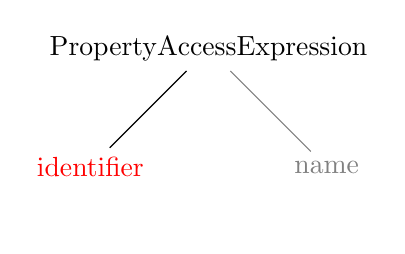
\begin{tikzpicture}
	\node {PropertyAccessExpression}
		child {node [red] {identifier}}
		child [white] {node [yshift = -0.5cm] {\phantom{node}}}  % ensure same height as sibling figures
		child [gray] {node [gray] {name}}
		;
\end{tikzpicture}
\caption[LoF entry]{
	Node pattern for a property access, such as in:

	\code{\lowlight{return }\uline{\lowlight{obj}.\highlight{prop}}\lowlight{;}}
}

	\end{subfigure}
	\hfill
	\begin{subfigure}[t]{.32\linewidth}
		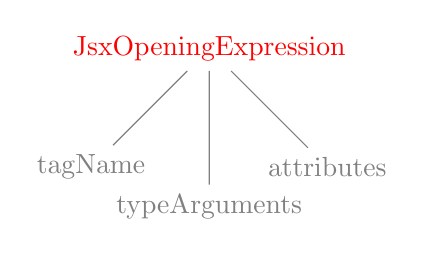
\begin{tikzpicture}
	\node [red] {JsxOpeningExpression}
		child [gray] {node [gray] {tagName}}
		child [gray] {node [gray, yshift = -0.5cm] {typeArguments}}
		child [gray] {node [gray] {attributes}};
\end{tikzpicture}
\caption[LoF entry]{
	Node pattern for a JSX opening tag, such as in:

	\code{\lowlight{elem = }\uline{<Button \lowlight{color}="\lowlight{blue}"> \lowlight{Google</Button>}}\lowlight{;}}
}

	\end{subfigure}

	\caption{Example AST patterns for TypeScript programs.
		The \highlight{highlighted} node contains the link to the declaration of the referenced identifier.
	}
	\label{fig:approach/mining/patterns}
\end{figure*}

Having downloaded the selected downstream dependency repositories, we can proceed to extract usage samples for the target package from each dependency repository.
Our goal is to identify these usage samples on a fine-granular level so that we can trace them down to the single identifiers that were exposed by the target package.

To do so, we start by parsing the source code of every dependency repository as well as the source of the target package each into a separate AST.

% TODO: use term "binding"?
In a second step, every dependency AST is traversed together with the target package AST in order to create links between semantically related nodes, e.g., between an expression and the variable it is assigned to, or between a function call and the definition of this function.

In the final step, we traverse the AST again and collect all nodes that are linked to a declaration in the target package.
To identify these links, we define a number of patterns for node structures and look up the declaration of every matched node (see \cref{fig:approach/mining/patterns}).

\subsection{Presentation of results}
\label{sec:approach/presentation}

After all references have been collected, a proper UI is still required to provide users easy access to these data that fulfills the requirements mentioned above.
To satisfy \cref{req2} and make our tool avaiable in the usual working environment of users, we implement it as an extension to a popular IDE.
One of the most popular IDEs that support JavaScript, and the one with the highest annual growth, is Visual Studio Code\footnote{\url{https://code.visualstudio.com/}}\footnote{Top IDE Index by Pierre Carbonnelle (2021): \url{https://pypl.github.io/IDE.html}}.
As it also provides a comprehensive set of APIs for extension developers, we have decided to roll our tool out as a VS Code extension.

For choosing appropriate views of the raw reference data, we have identified three common questions of package developers to answer each of which they require access to downstream dependencies and their usage samples:

\begin{enumerate}[label=Q\arabic*]
	\item Which dependencies do use the target package and what problems are they solving with it?
	\item By how many dependencies is a particular package member being used?
	\item In which contexts and constellations is a particular package member being used?
\end{enumerate}

To support developers in answering these questions and fulfill \cref{req1}, we have designed the following views for our extension:

\begin{enumerate}[label=(\roman*)]
	\item The \emph{dependency browser} allows to explore all downstream dependencies and, grouped for each dependency, all their references to the target package.
	\item The \emph{usage browser} displays all public package member and, grouped for each member, all dependencies and their references to this member.
	\item The \emph{CodeLens integration} provides quick access to a slice of the usage browser that is attached to the definition of each package member right in the source code editor.
\end{enumerate}

Both references and members are organized in a tree view reflecting the hierarchical structure of the original software repository.
In addition, we recognize the effort of browsing large lists of dependency data and encounter it by providing an ``I'm felling lucky'' button for every view that redirects the user to a random dependency resp. reference to gain a faster, unbiased impression of usage samples.

	\section{Data collection}
\label{sec:data_collection}

Foo!

	\section{Usage sample mining}
\label{sec:usage_mining}

\begin{figure*}
	\begin{minipage}{\linewidth}
		\newcommand\textlowlight[1]{\textcolor{gray}{#1}}
		\newcommand\texthighlight[1]{\textcolor{accent1}{#1}}
		\begin{center}
			\begin{subfigure}[t]{.32\linewidth}
				\begin{tikzpicture}
	\node {CallExpression}
		child {node [accent1] {identifier}}
		child [gray] {node [gray, yshift = -0.5cm] {typeArguments}}
		child [gray] {node [gray] {arguments}};
\end{tikzpicture}
\caption[LoF entry]{
	Node pattern for a TypeScript functional call, such as in:

	\code{\textlowlight{result = }\uline{\texthighlight{fun}<\textlowlight{T1}, \textlowlight{T2}>(\textlowlight{arg1}, \textlowlight{arg2})}\textlowlight{;}}
}

			\end{subfigure}
			\hfill
			\begin{subfigure}[t]{.32\linewidth}
				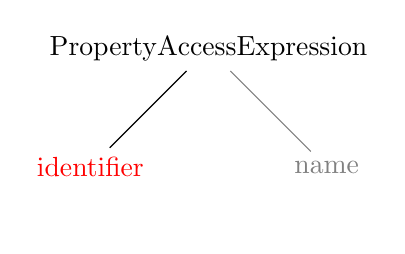
\begin{tikzpicture}
	\node {PropertyAccessExpression}
		child {node [red] {identifier}}
		child [white] {node [yshift = -0.5cm] {\phantom{node}}}  % ensure same height as sibling figures
		child [gray] {node [gray] {name}}
		;
\end{tikzpicture}
\caption[LoF entry]{
	Node pattern for a property access, such as in:

	\code{\lowlight{return }\uline{\lowlight{obj}.\highlight{prop}}\lowlight{;}}
}

			\end{subfigure}
			\hfill
			\begin{subfigure}[t]{.32\linewidth}
				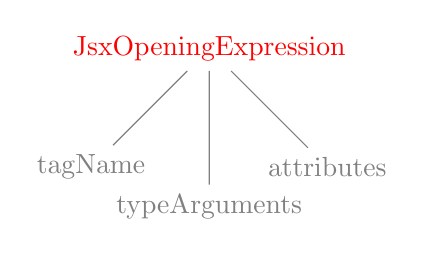
\begin{tikzpicture}
	\node [red] {JsxOpeningExpression}
		child [gray] {node [gray] {tagName}}
		child [gray] {node [gray, yshift = -0.5cm] {typeArguments}}
		child [gray] {node [gray] {attributes}};
\end{tikzpicture}
\caption[LoF entry]{
	Node pattern for a JSX opening element (as supported in React\protect\footnotemark{} or TypeScript\protect\footnotemark{}), such as in:
	\code{\lowlight{elem = }\uline{<Button \lowlight{color}="\lowlight{blue}"> \lowlight{Google</Button>}}\lowlight{;}}
}

			\end{subfigure}

			\caption{AST patterns for example JavaScript/TypeScript expressions.
				The \texthighlight{highlighted} node contains the link to the declaration of the referenced identifier.
			}
			\label{fig:usage_mining/patterns}
		\end{center}
	\end{minipage}
\end{figure*}

Having downloaded the selected downstream dependency repositories, we can proceed to extract usage samples for the target package from each dependency repository.
Our goal is to identify these usage samples on a fine-granular level so that we can trace them down to the single identifiers that were exposed by the target package.

To do so, we start by parsing the source code of every dependency repository as well as the source code of the target package each into a separate abstract syntax forest (ASF, i.e., a set of ASTs).

In a second step, a static type analysis is performed against each dependency ASF together with the target package's ASF.
The results of the type analysis are attached to the ASF so that every identifier is annotated with a type symbol that links to the declaration of the type for the identifier.
For instance, after this step, every variable node will contain a link to the assignment node of this variable, and every function call expression will contain a link to the definition of this function. \TODO{Give example?}
The operating principle of this type analysis depends on the kind of programming language; i.e., in statically typed languages, type symbols can usually be retrieved from the declaration of an identifier, whereas in dynamically typed languages, a control flow analysis will be required to identify the origin of every identifier's type.

In the final step, from each ASF all nodes are collected whose type is declared in the target package.
To identify these links, we define a set of language-specific patterns for AST subtrees that constitute a usage expression.
In particular, each of these patterns expects a node containing a link to an identifier declaration (see \cref{fig:usage_mining/patterns}).

The complete procedure is displayed in \cref{alg:usage_mining}.

\begin{algorithm}
	\caption{Extraction of usage samples.}\label{alg:usage_mining}

	\KwIn{\\\Indp
		$\mli{pkg}$: target package \\
		$\mli{dependencies}$: downstream dependencies}
	\KwOut{usage samples (set of strings)}
	\;
	\For{$\mli{dep} \in \mli{dependencies}$}{
		$\mli{asf} \gets \mtx{parse}(\mli{dep} \cup \mli{pkg})$\;
	  	$\mtx{annotate\_types}(\mli{asf})$\;
		\For{$\mli{ast} \in \mli{asf}$}{
			\For{$\mli{node} \in \mli{dfs}(\mli{ast})$}{
				\For{$\mli{pattern} \in \mli{patterns}$}{
					\If{$\mli{pattern}.\mtx{matches}(\mli{node}) \wedge \mli{pkg}.\mtx{declares}(\mli{pattern}.\mtx{getType}(\mli{node}))$}{
						\kwYield{$\mli{node}.\mtx{text}$}
					}
				}
			}
		}
	}
\end{algorithm}

	\section{Presentation of results}
\label{sec:presentation}

Foo!

	\section{Evaluation}
\label{sec:evaluation}

To evaluate the efficacy of our approach, we formulate three research questions:

\begin{enumerate}[label=RQ\arabic*]
	\item \label[requirement]{resqu1} What is the quality and quantity of the proposed approaches for dependency collection?
	\item \label[requirement]{resqu2} What is the quality and quantity of the proposed approach for mining usage samples?
	\item \label[requirement]{resqu3} How well is the proposed tool applicable?
\end{enumerate}

In the following, we are going to investigate each of these questions.

\subsection{\ref{resqu1}: Dependency collection}
\label{sec:evaluation/resqu1}

To assess the quality of dependency collection, we analyze it with respect to extent, precision, recall, and performance.
\Cref{tab:evaluation/resqu1/quantities} shows the number of dependencies that were collected from each data source following the proposed approaches for a set of arbitrarily selected npm packages.
For each package, we have annotated a subset of the collected dependencies (max. 20 dependencies per package) manually to identify and classify false positive hits.

\begin{table}
	\centering
	\small
	\setlength\tabcolsep{4pt}

\begin{tabular}{lrrrrrr}
	\multirowthead{2}{Package} &
		\multirowthead{2}{GitHub \\ stars} &
		\multicolumn{2}{c}{npm} &
		\multicolumn{2}{c}{Sourcegraph} &
		\multirowthead{2}{Intersection \\{} [\si{\percent}]} \\
	%
		&
		&
		\thead{count} &
		\thead{FPR} &
		\thead{count} &
		\thead{FPR} &
	\\
	\hline
	base64id	& 16	& 72	& 0.2	& 45	& 1	& 0.08 \\
	nemo	& 38	& 1	& 0	& 1	& 1	& 0 \\
	random-js	& 556	& 219	& 0.14	& 193	& 0.36	& 0.15 \\
	\makecell{kubernetes-\\client}	& 902	& 36	& 0.13	& 79	& 0.21	& 0.16 \\
	jsonschema	& 1,547	& 394	& 0	& 517	& 0.18	& 0.02 \\
	graphql	& 18,005	& 396	& 0.17	& 8,863	& 0.68	& 0.02 \\
	cheerio	& 24,228	& 396	& 0.07	& 8,863	& 0.07	& 0.00 \\
\end{tabular}

	\caption{Quantity and false-positive rates (FPR) of downstream dependencies found by both approaches for selected packages.}
	\label{tab:evaluation/resqu1/quantities}
\end{table}

\subsubsection{Extent}
\label{sec:evaluation/resqu1/extent}

Regarding the total number of dependencies collected by each approach, no clear trend in favor of any approach can be ascertained for small or medium packages (having less than 10,000 stars on GitHub).
For larger packages (having at least 10,000 stars), however, the number of dependencies collected from the npm registry stagnates near to 400 hits; beyond this limit, the npm registry will return internal server errors only.
For Sourcegraph, on the other hand, we have not hit any limitations so far; currently, they do not provide any official documentation for the exact rate limits.

As the disjunct proportion of results from both approaches is very small (on average about \SI{6}{\percent}), we consider a combination of both data sources useful for maximizing the extent and diversity of the gained dataset.

\subsubsection{Precision}
\label{sec:evaluation/resqu1/precision}

The precision of collected dependencies is drastically lower for dependencies found on Sourcegraph than for such found on npm.
\Cref{fig:evaluation/resqu1/fp_causes} collates the causes we have identified for these false positives; most frequently, repositories specify a dependency on the target package in their package manifest file but do not actually import this package at any place.

\begin{figure}
	\centering
	\small
	\begin{bchart}[steps={0.1,0.2,0.3,0.4,0.5},max=0.5,width=4.5cm]
	\bcbar[color=bchart.accent1]{0.385}
	\bclabel{package unused}
	\bcbar[color=bchart.accent2]{0.269}
	\smallskip
	\bcbar[color=bchart.accent1]{0.277}
	\bclabel{peer dependency}
	\bcbar[color=bchart.accent2]{0.077}
	\smallskip
	\bcbar[color=bchart.accent1]{0.015}
	\bclabel{type definitions only}
	\bcbar[color=bchart.accent2]{0.115}
	\smallskip
	\bcbar[color=bchart.accent1]{0.015}
	\bclabel{\code{package.json} mismatch}
	\bcbar[color=bchart.accent2]{0}

	\bclegend{3pt}{bchart.accent1/Sourcegraph,bchart.accent2/npm}
\end{bchart}

	\caption{Causes for false-positive dependency matches and their frequencies.}
	\label{fig:evaluation/resqu1/fp_causes}
\end{figure}

In some situations, this may happen if the package is a plugin for another package or if it is invoked as a CLI from a build script (\TODO{C'mon, we could improve data classification for this}), but in the majority of repositories, developers trivially appear to have specified the upstream dependency by accident (e.g., while copying a \code{package.json} file over from another package), or to have forgotten to remove the upstream dependency after switching away from using the package.
Rarer causes include repositories that only add type definitions for TypeScript to a package but do not actually import it, as well as, especially for repositories found on Sourcegraph, other packages required by a repository declaring a peer dependency on the target package which needs to be fulfilled by the depending repository.

We explain the increased false-positive rate for Sourcegraph dependencies by our observation that packages found on npm typically stand out by their higher cohesion and professional maintenance, whereas GitHub projects are more likely run as imperfect hobby projects.

We stress that a reduced precision does not impair the quality of results displayed to package developers as all dependencies not containing at least one
usage sample can be easily filtered out, but downloading and analyzing any irrelevant packages lowers the performance of the approach.

\subsubsection{Recall}
\label{sec:evaluation/resqu1/recall}

Besides the precision of collected dependencies, their recall is also of interest.
As the dependencies are collected from two giant datasets in extracts only, a quantitative analysis of false-negative hits based on manual annotation of these datasets would be too expensive for this paper.
Nevertheless, there are some causes that will prevent a dependency from being found by our approaches:

\begin{itemize}
	\item Packages without a proper dependency manifest cannot be detected by our approaches which are based on exactly these metadata.
	\item On npm, naturally packages only will be found, creating a bias towards rather generic and professional software.
	\item On both platforms, results will be sorted based on intransparent criteria (which, as we however speculate, include the number of direct dependents on npm and the recent update frequency on Sourcegraph, resp.).
		As we only fetch the first dependencies from both data sources, this sorting is a likely source of further biases.
		These biases could be fought by always fetching all dependencies, but this would drastically reduce the overall performance.
\end{itemize}

\subsubsection{Performance}
\label{sec:evaluation/resqu1/performance}

\begin{table}
	\centering
	\small
	\begin{threeparttable}
		\begin{tabular}{lrr}
	\toprule
	\thead{Metric}	& \thead{npm}	& \thead{Sourcegraph} \\
	\midrule
	API limitations	& max. 400 results	& none known \\
	search speed%
		\alphtnote{1}
		[\si{\second/pkg}]
		& 1.58	& 0.04 \\
	download speed%
		\alphtnote{1}\alphtnote{2}
		[\si{\second/pkg}]
		& 0.26	& 8.80 \\
	ROM [\si{\mega\byte}/pkg]
		& 5.8	& 27.2 \\
	\bottomrule
\end{tabular}

		\begin{tablenotes}
			\footnotesize
			\item[\alphtnotetext{1}] Hardware specifications of the test machine: 7 vCPUs Intel Xeon Cascade Lake @ \si{2.80}{GHz}, internet downspeed ~1.8 \si{Gbit}/\si{s}.
			\item[\alphtnotetext{2}] Effective speed while downloading multiple packages in parallel.
		\end{tablenotes}
	\end{threeparttable}

	\caption{Key performance metrics for both dependency collection methods.}
	\label{tab:evaluation/resqu1/performance}
\end{table}

\Cref{tab:evaluation/resqu1/performance} gives some basic metrics comparing the performance of both data sources.
While searching downstream dependencies is slower by average on npm as we use a web scraper instead of an API for this source, npm packages are usually smaller as opposed to many monorepos on OSS platforms that contain multiple node.js packages, and they are faster to download since the download-git-repo package that we use for repositories found on Sourcegraph, as of today, only uses zipballs instead of tarballs while the latter would offer a higher compression rate.

\subsection{\ref{resqu2}: Usage mining}
\label{sec:evaluation/resqu2}

To assess the quality of usage mining, we examine the precision, recall, and performance of this processing step.
Due to the complexity of a detailed annotation process, we only consider the existence of found usage samples on the dependency level.
The absolute quantity of found usage samples varies largely for different packages and dependencies based on the semantic extent of the package and the coupling between package and dependency.

\subsubsection{Precision}
\label{sec:evaluation/resqu2/precision}

Under laboratory conditions, false-positive usage samples cannot be emitted by our approach if we assume the correctness of the TypeScript compiler.
There are only two exceptions to this invariant:
\begin{enumerate*}[label=(\roman*)]
	\item If there is a name collision between two packages, invalid or false positives usage samples may be emitted.
		However, the npm infrastructure attempts to rule out these collisions by using the package name as a unique ID for every published package.
	\item If dependency developers deliberately interfere with the TypeScript compiler (for instance, by suppressing type errors using a \verb|@ts-ignore| comment\footnote{\url{https://www.typescriptlang.org/docs/handbook/release-notes/typescript-2-6.html\#suppress-errors-in-ts-files-using--ts-ignore-comments}}), both false positive and false negative matches are possible.
\end{enumerate*}

\subsubsection{Recall}
\label{sec:evaluation/resqu2/recall}

To evaluate the recall of our approach, we have refined the experimental dataset collected in \cref{sec:evaluation/resqu1} and removed all false-positive dependencies.
Within this cleansed dataset, the overall rate of dependencies for that our approach is unable to find at least one usage sample accounts for \SI{47.9}{\percent}.
As a cause for these false negatives, we have identified a number of systematic causes:

\begin{itemize}
	\item Many projects on OSS platforms have complex build configurations that include additional transpilation or code generation steps before a final version of the source code is reached that is valid to the node.js interpreter or the TypeScript compiler.
		Unless we add explicit support for such build configurations, type analysis and thus usage mining for these projects will fail.
	\item In some situations, additional type definitions are required to perform a complete type inference of a dependency.
		This is the case for every parametrized callback from a package for that type definitions are not available.
		This limitation could be resolved by downloading or generating the type definitions for all upstream dependencies of every downstream dependency; this, on the other hand, would reduce the performance of the approach.
	\item In general, the static type analyzer of TypeScript has its limitations.
		For instance, the type analysis will have a limited recall for certain control flow patterns or metaprogramming constructs such as meta-circular evaluation using the the \code{eval()} function or dynamic function binding using \code{Function.bind()} and friends.
\end{itemize}

\subsubsection{Performance}
\label{sec:evaluation/resqu2/performance}

The total time spent for performing type analysis for a repository from the experimental dataset and mining usage samples averages ca. \num{3} seconds.
The complete ASF of an average parsed repository consumes between \SI{10}{MB} and \SI{500}{MB} of RAM, depending on the size of the analyzed repository.

\subsection{\ref{resqu3}: Tool}
\label{sec:evaluation/resqu3}

To assess the applicability of our proposed tool, we investigate the different options of users who would like to answer the questions raised in \cref{sec:framework}.
We further analyze how far our tool meets the requirements posed above.

\subsubsection{Answering user questions}

In order to answer \cref{q1} without our tool, it would be possible to access the aforementioned data sources manually.
Both npm and Sourcegraph provide suitable web interfaces for surveying dependent packages or search results, resp.
To understand the intent of a dependency, users can read its documentation online, if any, or browse its implementation.
The source code of repositories can be browsed on Sourcegraph, but on npm, this is not possible, and users need to either manually download and extract the package or follow the link to an open-source code repository if the package provides one.

With our tool, the data collection process is condensed into a single button that displays all references from both data sources incrementally.
Users can hover or click any dependency to view its documentation or implementation.

In order to answer \cref{q2,q3} without our tool, users need to scan each dependency found in the previous step separately to count or read all usage samples, resp.
If they are intending to analyze the usage of a member with an unambiguous name, they can perform an expeditious string search.
For repositories found on Sourcegraph, this is either possible by starting a new search on the platform or by searching the source code in the original code host.
If the source code is not available online, it needs to be downloaded first and searched locally.
If the member of interest has a confusable name, a string search could not lead to the desired result.
In this case, users need to download and install the project and view it in an IDE that supports reference search (for instance, there is a built-in feature for this in VS Code).
Alternatively, they can try to use the precise code intelligence mode on Sourcegraph (see \cref{sec:related_work/usage_samples}).
However, as of today, precise code intelligence is only available for a small number of repositories as both the dependent repository and the dependency repository are required to provide a special index file.

Within our tool, all usage samples can be collected automatically and be merged into a single list.
Once the collected dependencies have been processed, users can select a member of interest and view all its usage samples with a single click.
For the usage analysis of Java APIs, there is also the tool \caps{Exapus}\citep{de2013multi} which differentiates between different kinds of member usages such as instantiation of vs. inheritance of a class.
Such a classification mechanism could also improve the usability of our tool

\subsubsection{Meeting requirements}

We break down \cref{req1} into three acceptance criteria: application liveness, small resource footprint, and easy setup.

As a result of the numbers mentioned in the evaluation of the previous research questions, our tool is able to process 5 up to 12 dependencies per minute while requiring about \SI{500}{MB} RAM in total and less than \SI{30}{MB} ROM per package.
I.e., from the moment the tool is activated, the first results usually take less than 10 seconds to appear on the UI.
This is an acceptable delay with regard to Shneiderman's definition of acceptable application response times, so the liveness criterion is fulfilled.\footnote{Ben Shneiderman and Catherine Plaisant. 2010. Designing the user interface: Strategies for effective human-computer interaction. Pearson Education India.}
Even if the tool is run for 10 minutes, it will occupy less than \SI{4}{GB} of ROM that can be released at any time, which we consider a small resource footprint at a time where modern operating systems require at least \SI{64}{GB} ROM; thus, also the second acceptance criterion is fulfilled.
As our extension can be installed with two clicks from the Visual Studio Code Extension Marketplace, it is also easy to set up and thus fulfills the first requirement.

\Cref{req2} effectively calls for a minimum number of context switches that are required to use the tool, i.e., for minimizing the temporal, spatial, and semantic distance\footnote{David Ungar, Henry Lieberman, and Christopher Fry. 1997. Debugging and the experience of immediacy. Commun. ACM 40, 4 (1997), 38–43.} between the downstream dependency UI and the IDE used by package developers.

Once the data are available in the UI, interaction with them is possible with the same speed as with local source files in the package.
This is compatible with Shneiderman's requirement to frequent tasks and indicates a low temporal distance.

The spatial distance varies for the different views of the tool:
For the dependency browser and the usage browser, a separate toolbar has to be opened, which indicates a higher spatial distance; still, the artifacts are available in the same IDE.
On the other hand, the dependency artifacts were not displayed in the IDE without our tool and have no strong relationship to the already existing artifacts, so any closer integration into an existing view would increase unintended coupling between independent domains.
The code annotations are very close to the original source code and thus have a small spatial distance.

The semantic distance can be described as the perceived similarity of artifacts displayed both in the tool's UI and in the existing IDE.
Such artifacts are the package and dependency members displayed in the usage browser of our tool.
Most items in the usage browser bear the same label as the corresponding identifier in the source code, which reduces the semantic distance.
However, some nodes in the path of dependency members correspond to anonymous expressions in the source code that do not bear a label themselves and thus are labeled using a generic fallback token in our tool (see \cref{fig:implementation/presentation/screenshot/dependency_browser}).
This does not match the labeling convention in VS Code (as displayed in the outline view of the explorer activity bar), where a target identifier is determined from the context of the expression.
For such nodes, the current semantic distance of our tool is still higher than necessary.

With a low temporal distance, a low-to-medium spatial distance, and a mainly low semantic distance, our tool also fulfills \cref{req2}.

	\section{Conclusion and future work}
\label{sec:conclusion}

Foo!

future work:

* evaluation as future work:

	- rq2 - false negatives durch annotation ermitteln
	- rq3 - user study

* pattern analysis -> sample classification, potential for reuse
* dynamic analysis -> parameter/return value insights, coverage detection
* dependency classification/clustering through metrics (number of references, coupling)

minor:
* support more AST pattern (e.g. import())

STEHENGEBLIEBEN: Notizen hierfür, in slides übernehmen, dann weitere Notizen für Präsi anwenden. Heute nochmal durchsprehcne?


	\begin{acks}
%To Robert, for the bagels and explaining CMYK and color spaces.
\end{acks}


	\bibliographystyle{ACM-Reference-Format}
\bibliography{paper}


	%\appendix

\end{document}
\endinput
